\documentclass[tikz,border=4pt]{standalone}
\usepackage[T1]{fontenc}
\usepackage{mathptmx}
\usetikzlibrary{arrows.meta,calc}
\begin{document}
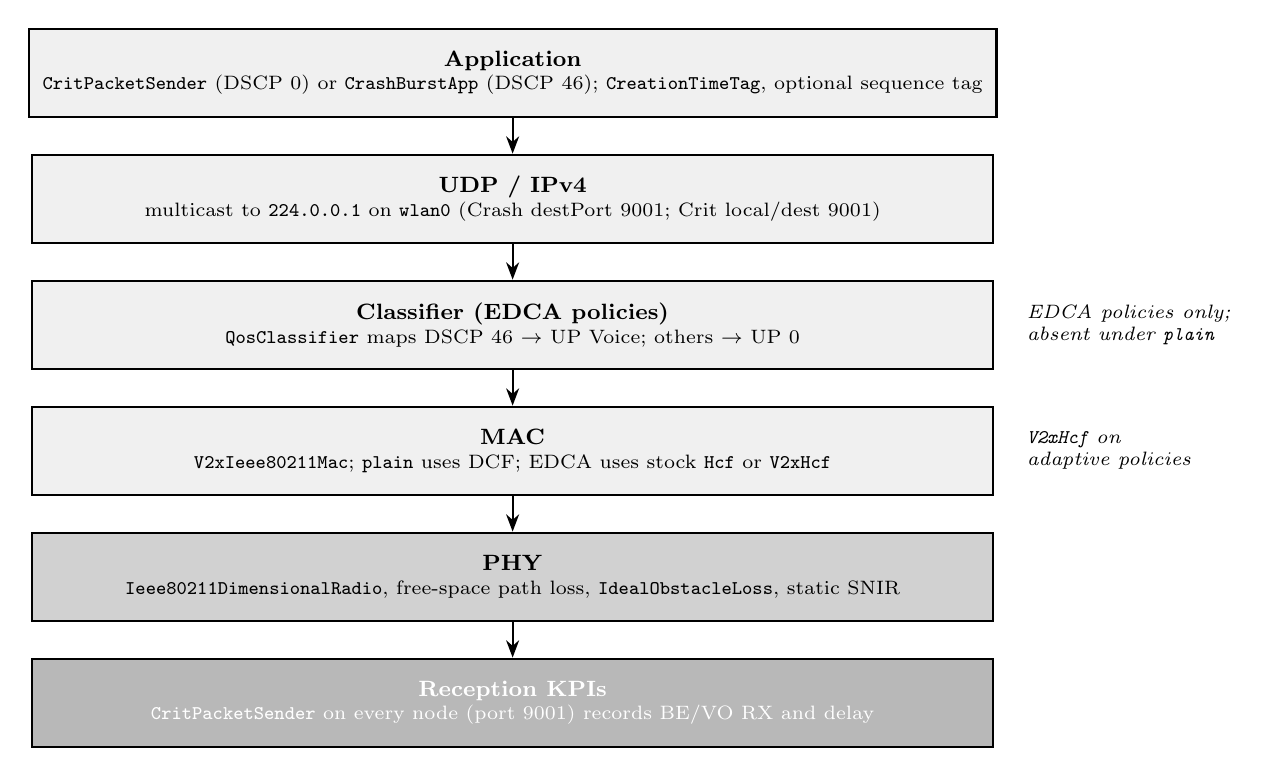
\begin{tikzpicture}[
  font=\footnotesize,
  >=Stealth,
  thick,
  box/.style={draw, thick, align=center, inner sep=5pt, minimum width=12.2cm},
  layer/.style={box, fill=black!6, minimum height=1.12cm},
  phy/.style={box, fill=black!18, minimum height=1.12cm},
  kpi/.style={box, fill=black!28, text=white, minimum height=1.12cm},
  lbl/.style={font=\scriptsize\itshape, align=center},
  arr/.style={-{Stealth[length=2.2mm]}, thick},
]
  \node[layer] (app) at (0,8.00) {%
    \textbf{Application}\\[-1pt]
    {\scriptsize \texttt{CritPacketSender} (DSCP~0) or \texttt{CrashBurstApp} (DSCP~46);
     \texttt{CreationTimeTag}, optional sequence tag}};
  \node[layer] (udp) at (0,6.40) {%
    \textbf{UDP / IPv4}\\[-1pt]
    {\scriptsize multicast to \texttt{224.0.0.1} on \texttt{wlan0}
     (Crash destPort~9001; Crit local/dest~9001)}};
  \node[layer] (clf) at (0,4.80) {%
    \textbf{Classifier (EDCA policies)}\\[-1pt]
    {\scriptsize \texttt{QosClassifier} maps DSCP~46~$\rightarrow$~UP Voice; others~$\rightarrow$~UP~0}};
  \node[layer] (mac) at (0,3.20) {%
    \textbf{MAC}\\[-1pt]
    {\scriptsize \texttt{V2xIeee80211Mac}; \texttt{plain} uses DCF; EDCA uses stock \texttt{Hcf} or \texttt{V2xHcf}}};
  \node[phy]  (phy) at (0,1.60) {%
    \textbf{PHY}\\[-1pt]
    {\scriptsize \texttt{Ieee80211DimensionalRadio}, free-space path loss, \texttt{IdealObstacleLoss}, static SNIR}};
  \node[kpi]  (rx)  at (0,0.00) {%
    \textbf{Reception KPIs}\\[-1pt]
    {\scriptsize \texttt{CritPacketSender} on every node (port~9001) records BE/VO RX and delay}};

  \draw[arr] (app.south) -- (udp.north);
  \draw[arr] (udp.south) -- (clf.north);
  \draw[arr] (clf.south) -- (mac.north);
  \draw[arr] (mac.south) -- (phy.north);
  \draw[arr] (phy.south) -- (rx.north);

  \node[lbl, anchor=west, align=left] at (6.40,4.80)
    {EDCA policies only;\\absent under \texttt{plain}};
  \node[lbl, anchor=west, align=left] at (6.40,3.20)
    {\texttt{V2xHcf} on\\adaptive policies};
\end{tikzpicture}
\end{document}
